\chapter{Future Work}

We have presented preliminary results of visual spatiotemporal social media data analytics techniques for detection and examination of abnormal events, spatial decision support in crisis management, and anomalous human movement analysis.
%Thus far, the proposed techniques can be utilized in real-time or post-event analysis.
In emergency management and response, it is important to not only analyze what happened in the past and what is occurring in the present, but also predict what might arise in the future.
This can be done by using historical data and relevant context information to model and extrapolate future situations.
It is useful to know how current situations may change or when and where new situations may arise in the future.
This allows the emergency response to be more proactive instead of passive.
Although automated techniques are useful, user-guided controls can be applied to enhance the techniques.
This is because the accuracy is not guaranteed and unexpected situations should be taken into account.
In this context, as future work, we plan to develop predictive and interactive analytics techniques based on spatiotemporal social media data for integrating visual analytics approaches with automated data analysis models for predicting human movements.
The following sections describe in detail our plan of future study and a time line scheduled.

\section{Design of a Prediction Model using Historical Trajectory}
\label{sec:prediction_model}

Research on predicting human movements has attracted a lot of attention in recent years~\cite{Cho:2011:FAM,Jiang:2009:Ranking,Lin:2013:Predicting}.
The existing techniques have mainly focused on finding the next place of an individual based on the observations of his or her past movement patterns or frequent behaviors of similar users~\cite{Asahara:2011:PMP,Gambs:2012:NPP}.
In this work, we will focus on predicting overall flow of group movements.
We plan to design a model for predictive Vector Fields (VFs) based on spatiotemporal social media data, which is motivated by wind vector field maps.
An example of wind vector field map is shown in Figure~\ref{fig:wind}.
\begin{figure}[th]
	\centering
	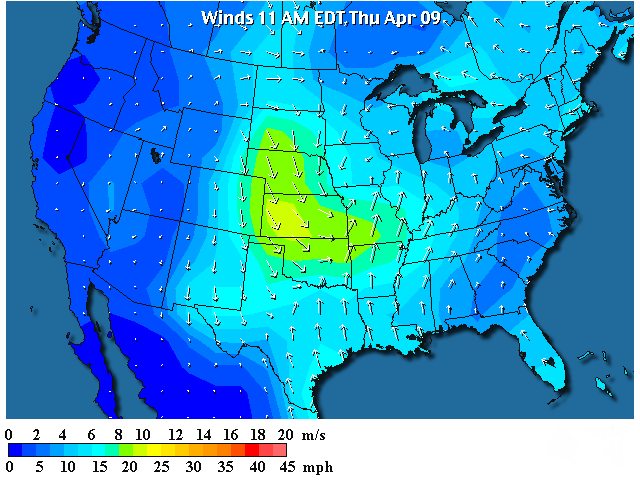
\includegraphics[width=0.8\linewidth]{wind_vector_field}
	\caption{Wind vector field map over the US~\cite{Weather:2015:Wind}.}
	\label{fig:wind}
\end{figure}

\textbf{Vector Field Generation:} 
The planned process of trajectory-based VF generation is the following:
%1) Generating trajectories for a specific time frame on a 2D space, 
%2) Dividing the trajectory space into sub-spaces on a grid, 
%3) For each cell, transforming the trajectories passing through the cell to vectors and calculating the sum of the vectors, and 
%4) Generating VFs using the sum vectors of each cell for the movements within the specific time frame.
\begin{enumerate}[label={(\arabic*)}]
	\item Generating trajectories of a specific time frame on a 2D space.
	\item Dividing the space of trajectories into sub-spaces on a grid.
	\item For each cell, transforming the trajectories passing through the cell into vectors and calculating the sum of the vectors.
	\item Generating vector fields using the sum vectors of each cell for visualizing the movement flow within a specific time frame.
\end{enumerate}
An initial result is shown in Figure~\ref{fig:vector_field} where the sample trajectories were generated around around the finish line at the Boston Marathon 2013 during 12 hours after the explosions.

\textbf{Vector Field Prediction:} 
The planned process of the future VFs prediction is the following:
\begin{enumerate}[label={(\arabic*)}]
	\item Creating a series of VFs for a certain past period of time frames,
	\item Extracting a series of vectors from the cells with a same coordinate from the series of VFs,
	\item Generating two time series, directions and magnitudes, of the series of vectors,
	\item Applying a temporal prediction method to the two time series for predicting the direction and the magnitude of the future vector of the coordinate, and
	\item Repeating the same procedure on each coordinate to create the future VFs.
\end{enumerate}
Figure~\ref{fig:vector_prediction} shows the overall procedure of our vector field prediction.

However, the VFs generated by traditional sum vectors have a limitation in representing flow of movements in specific cases.
For example, if there are two same size vectors pointing in opposite directions in a cell, the sum vector becomes a zero vector.
To mitigate this drawback, we will extract multiple dominant vectors based on the distribution of the vectors in a cell.
For temporal prediction methods of the time series, if the time series exhibit regular patterns (e.g., daily, weekly, monthly), the STL which is described in Section~\ref{subsec:filtering} will be a promising prediction method.
Also, our prediction model can be utilized to detect unusual movement flow in real-time by comparing actual real-time flow to the predicted one.

%Also, we will evaluate and improve our prediction model by using our about three years data.
%The cell is divided into the same number of sub-cells.
%The multiple dominant vectors are assigned to the sub-cells.

\begin{figure}[t]
	\centering
	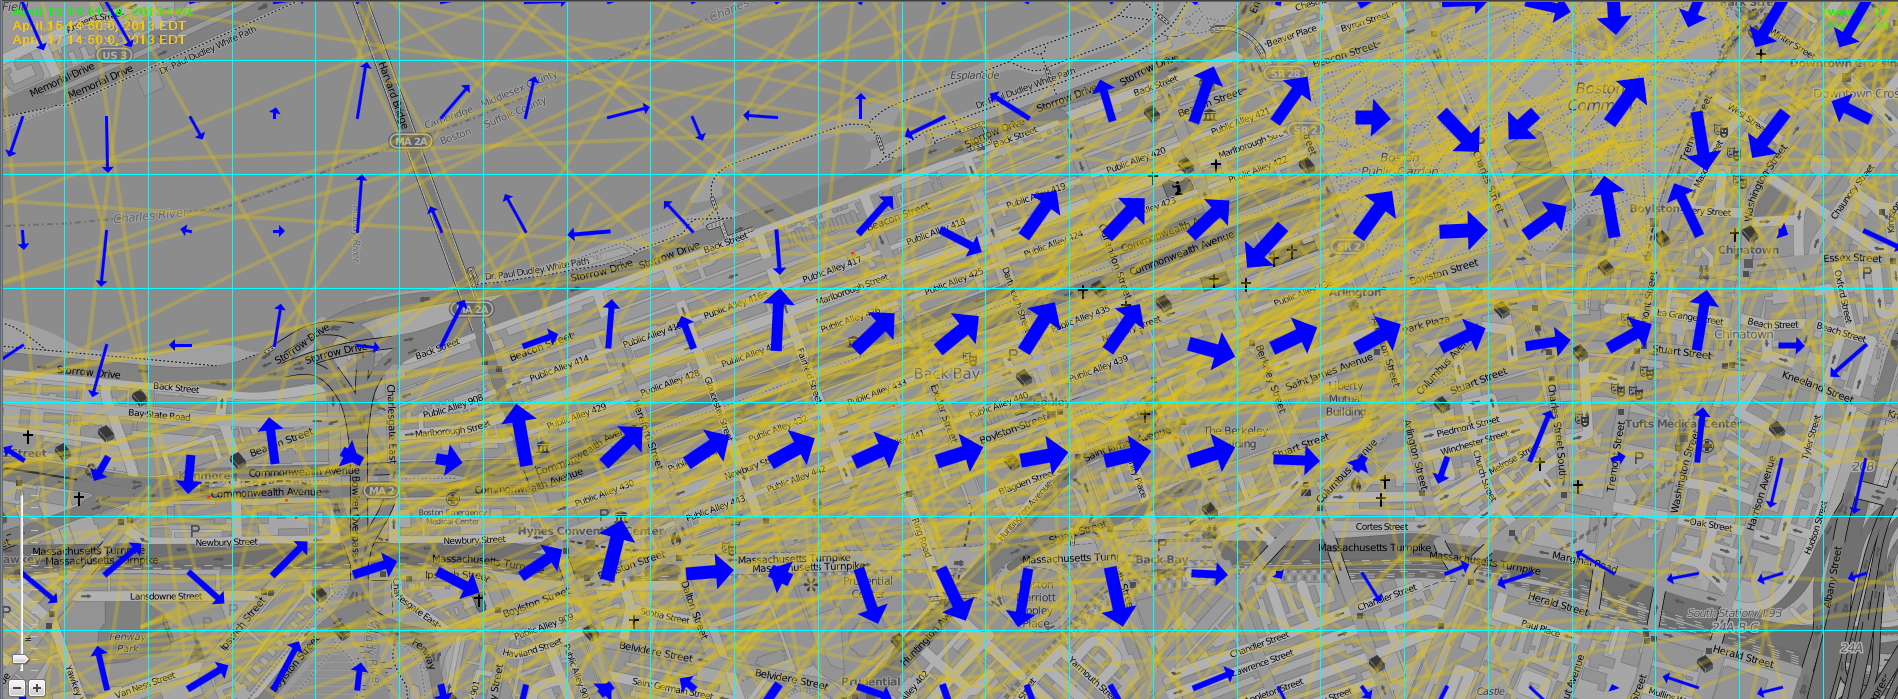
\includegraphics[width=1.0\linewidth]{CountasThicknessLengthasLength2}
	\caption{Initial results: vector field based on a trajectory space.}
	\label{fig:vector_field}
\end{figure}

\begin{figure}[t]
	\centering
	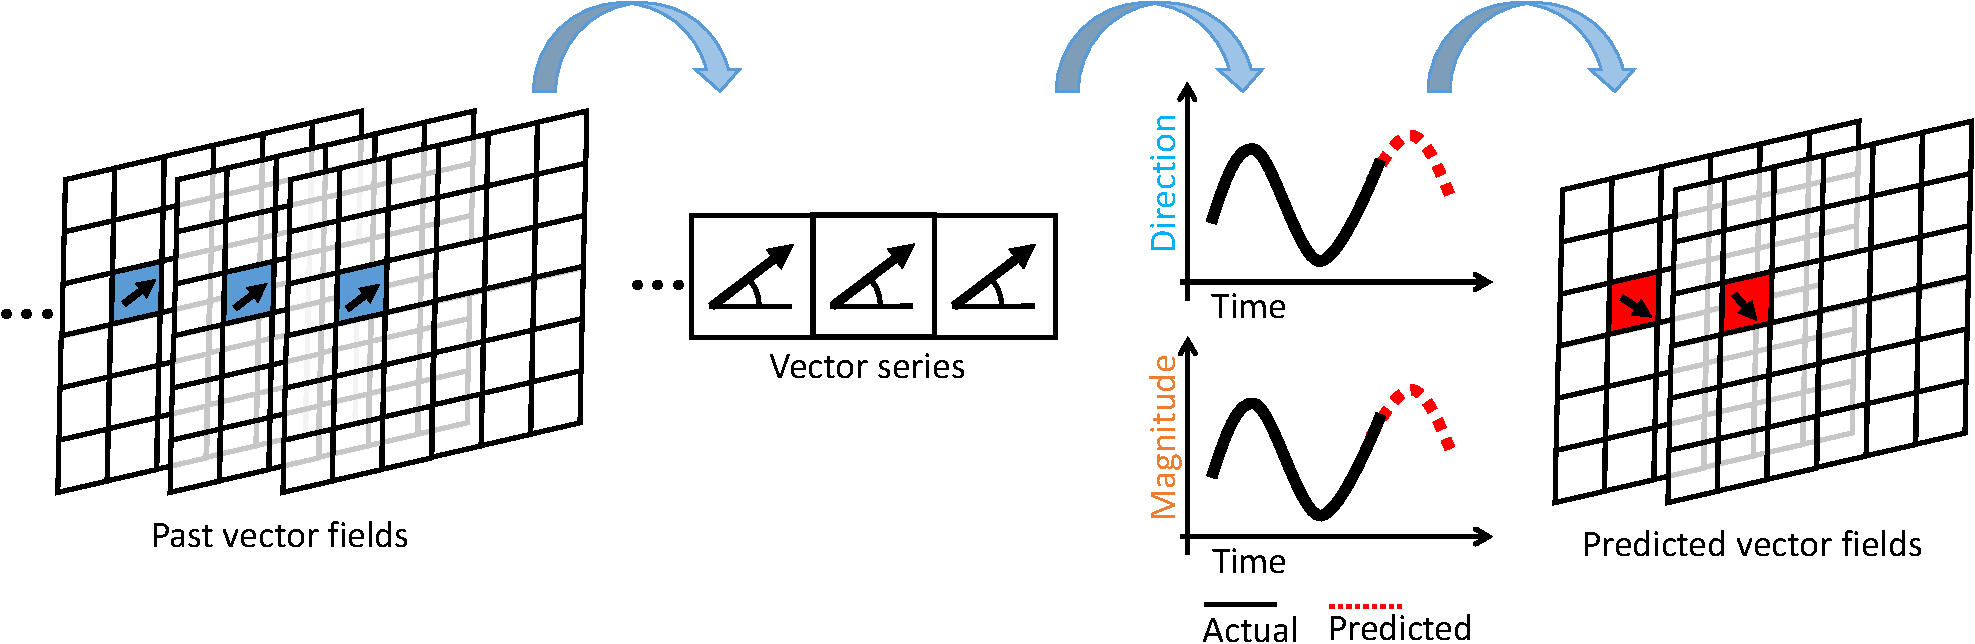
\includegraphics[width=1.0\linewidth]{vector_field_prediction}
	\caption{The process of vector field prediction}
	\label{fig:vector_prediction}
	%\vspace{-0.4cm}
\end{figure}

\textbf{Interactive Visualization:} 
%After calculating the predictive VFs generated by using the proposed prediction model, 
We plan to develop a visualization technique based on Line Integral Convolution (LIC)~\cite{Cabral:1993:Imaging}, a texture synthesis technique for flow visualization, to represent flow of the VFs (human movements).
%LIC is a texture synthesis technique for flow visualization.
%where it takes vector fields and a white noise image, convolves them to exploit spatial correlation in the flow direction.
%This technique takes a vector field and a white noise image, and convolves them in order to get something very similar to the images above.
While traditional LIC shows the streamlines of the vector fields, the directions of the vectors are not represented in the space.
To address this limitation, variations of LIC have been proposed, such as Animating Line Integral Convolution (ALIC) and Oriented Line Integral Convolution (OLIC)~\cite{Wegenkittl:1997:Animating,Wegenkittl:1997:Fast}.
Figure~\ref{fig:wind_isaac} shows an example of LIC visualization.
We will investigate and develop a LIC-based visualization technique to effectively visualize trajectory data.
%We will apply and test both visualization techniques (ALIC and OLIC) on our dataset.
We will develop a visual analytics system that provides interaction with not only the visualization, but also the back-end prediction model.


\begin{figure}[t]
	\centering
	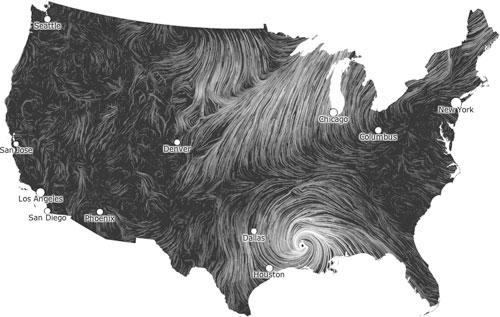
\includegraphics[width=0.8\linewidth]{wind_isaac_storm}
	\caption{LIC visualization showing wind flowing of Hurricane Isaac (September 2012) over the US
	%Zooming in south area (Bottom)
	~\cite{VW:2015:Windmap}.}
	\label{fig:wind_isaac}
	%\vspace{-0.4cm}
\end{figure}


\section{Integration of Context Information}

Human movements are affected by multiple factors including times of day (e.g., morning, evening), geographical features (e.g., school, bank), and specific events (e.g., sports game, festival).
%Researchers have worked on human movement mining using context information~\cite{Ying:2011:STM,Gonzalez:2008:UIH}.
Also, topics or keywords extracted from geo-tagged messages of a user can be utilized to infer the next place of the user.
In this context, we will investigate and design models using these context information to enhance the proposed prediction model described in Section~\ref{sec:prediction_model}.

Here is a possible virtual case study.
When an irregular event occurs, human movements may not conform to regular patterns.
For example, around a school campus, human mobility patterns on a sports game day evening may be different from the ones of a normal evening.
However, it will be able to pre-build a prediction model by leaning from past data of the same or similar events.
If so, we will detect the same or similar event on a specific day by the topic modeling described in Section~\ref{subsec:topic_extraction} and apply the pre-learned model for predicting the future movements.

\section{Evaluation}

We plan on performing evaluation of our prediction model using a large volume of historical data.
We have been collecting and storing Tweets on our database for more than three years since August, 2011.
To evaluate the prediction model, we will apply it to a variety of case studies including cases exhibiting regular patterns and abnormal patterns.
Also, we will evaluate our LIC-based visualization by comparing our technique with the existing visualization techniques for movement data (e.g., multiple poly-lines~\cite{Andrienko:2013:GroupMovement,Liao:2010:Anomaly} or series of arrows~\cite{Adrienko:2011:TrajAggregation,Andrienko:2007:Visual}).
%We will evaluate the prediction model based on datasets that exhibit either regular or irregular patterns in order to see robust 

%Also, we will evaluate and improve our prediction model by using our about three years data.

%\section{Interactive Visual Analytics System}

\section{Timeline}
%We schedule studies for the plans mentioned as future work in this proposal as following timeline:
Here is the expected schedule of the proposed future work as shown in Figure~\ref{fig:timeline}.
We will design a prediction model based on VFs using historical trajectory data from Summer 2015 and develop a LIC-based visualization technique during Fall 2015.
For enhancing our prediction model, we will start to develop a method by using context information in Fall 2015.
Finally, we will evaluate our prediction model and visualization technique in Spring 2016.

\begin{figure}[ht]
	\centering
	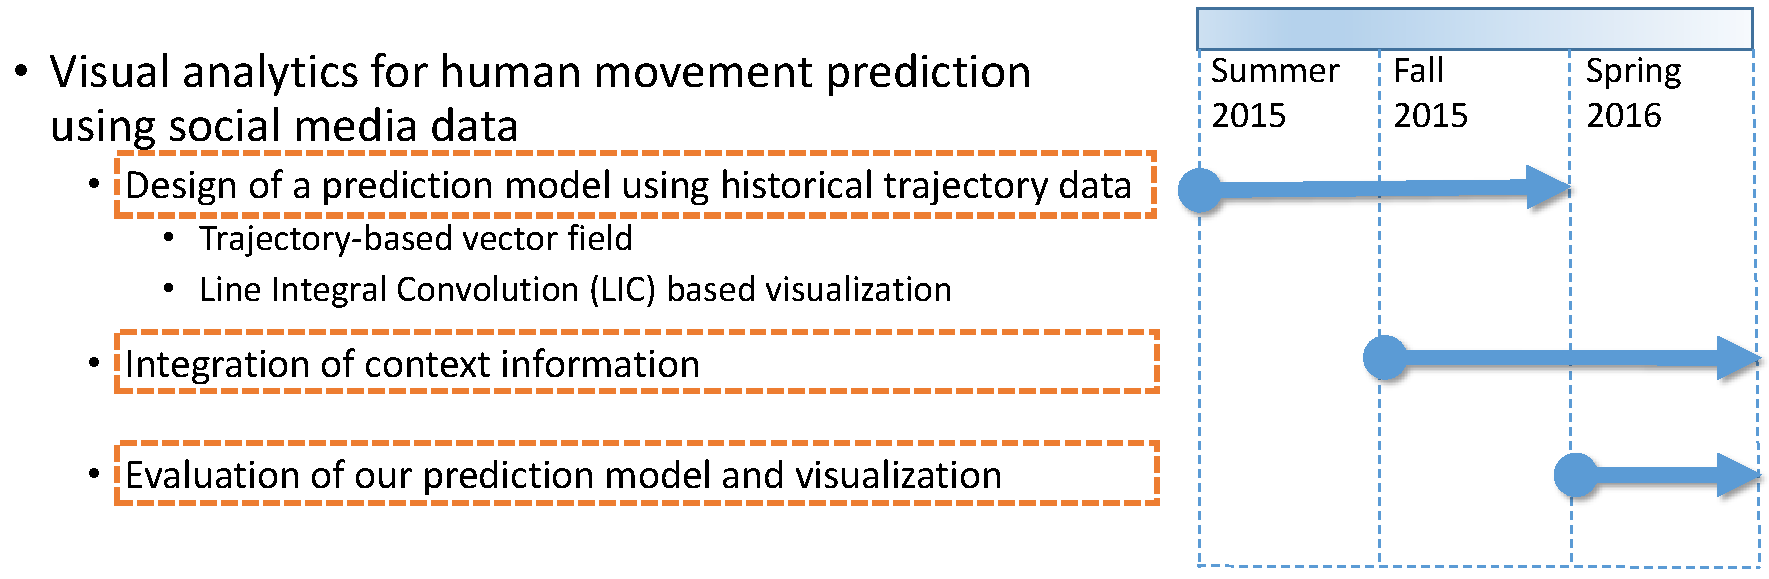
\includegraphics[width=1.0\linewidth]{timeline_v2}
	\caption{Proposed time line of future work}
	\label{fig:timeline}
\end{figure}




























